\documentclass[tikz,border=10pt]{standalone}
\usepackage{tikz}
\usetikzlibrary{calc, patterns, angles, quotes}

\begin{document}
	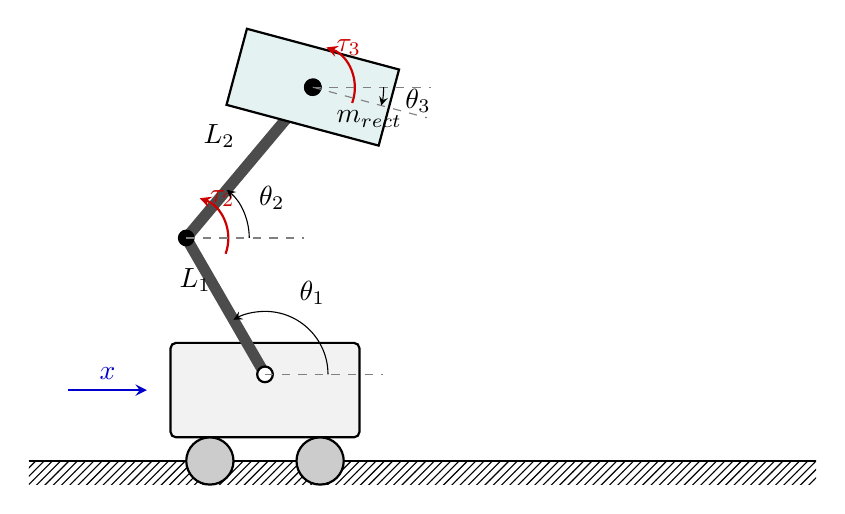
\begin{tikzpicture}[>=stealth, font=\sffamily]
		
		% --- Parametri Geometrici ---
		\def\cartW{2.4}
		\def\cartH{1.2}
		\def\wheelR{0.3}
		\def\Lone{2.0}
		\def\Ltwo{2.5}
		\def\rectW{2.0}
		\def\rectH{1.0}
		
		% Configurazioni angolari per il disegno
		\def\thetaOne{120}    % Angolo assoluto Link 1
		\def\thetaTwo{50}    % Angolo assoluto Link 2
		\def\thetaThree{-15} % Angolo assoluto Rettangolo
		
		% --- Stili ---
		\tikzset{
			cart/.style={draw=black, thick, fill=gray!10, rounded corners=2pt},
			link/.style={draw=black!70, line width=4pt, line cap=round},
			passive_joint/.style={circle, draw=black, fill=white, inner sep=2pt, thick},
			active_joint/.style={circle, draw=black, fill=black, inner sep=2pt},
			ground/.style={pattern=north east lines, draw=none},
			com/.style={circle, draw=black, inner sep=0pt, minimum size=6pt, fill=white, append after command={
					\pgfextra{
						\draw[fill=black] (\tikzlastnode.center) -- ++(0:3pt) arc(0:90:3pt) -- cycle;
						\draw[fill=black] (\tikzlastnode.center) -- ++(180:3pt) arc(180:270:3pt) -- cycle;
					}
			}}
		}
		
		% --- Piano di appoggio (Ground) ---
		\draw[thick] (-3, -\wheelR) -- (7, -\wheelR);
		\fill[ground] (-3, -\wheelR-0.3) rectangle (7, -\wheelR);
		
		% --- Carrello ---
		% Corpo del carrello
		\node[cart, minimum width=\cartW cm, minimum height=\cartH cm] (cart) at (0, \cartH/2) {};
		% Ruote
		\draw[thick, fill=gray!40] (-0.7, -\wheelR) circle (\wheelR);
		\draw[thick, fill=gray!40] (0.7, -\wheelR) circle (\wheelR);
		
		% Asse x (movimento carrello)
		\draw[->, thick, blue!80!black] (-2.5, \cartH/2) -- (-1.5, \cartH/2) node[above, midway] {$x$};
		
		% --- Coordinate dei Giunti ---
		\coordinate (J1) at (0, \cartH/2 + 0.2); 
		\coordinate (J2) at ($(J1) + (\thetaOne:\Lone)$);
		\coordinate (J3) at ($(J2) + (\thetaTwo:\Ltwo)$);
		
		% --- Links ---
		\draw[link] (J1) -- (J2) node[midway, above left, text=black] {$L_1$};
		\draw[link] (J2) -- (J3) node[midway, above left, text=black] {$L_2$};
		
		% --- End Effector (Rettangolo) ---
		\begin{scope}[shift={(J3)}, rotate=\thetaThree]
			% Corpo del rettangolo
			\draw[thick, fill=teal!10] (-\rectW/2, -\rectH/2) rectangle (\rectW/2, \rectH/2);
			
			% Simbolo del Centro di Massa
			\node[com, label={[label distance=4pt]below right:{$m_{rect}$}}] (com_rect) at (0,0) {};
		\end{scope}
		
		% --- Dettaglio Giunti e Coppie Attuatrici ---
		% Giunto 1: Passivo
		\node[passive_joint] at (J1) {};
		
		% Giunto 2: Attivo
		\node[active_joint] at (J2) {};
		\draw[->, thick, red!80!black] ($(J2)+(0.5, -0.2)$) arc (-20:70:0.55) node[right] {$\tau_2$};
		
		% Giunto 3: Attivo
		\node[active_joint] at (J3) {};
		\draw[->, thick, red!80!black] ($(J3)+(0.5, -0.2)$) arc (-20:70:0.55) node[right] {$\tau_3$};
		
		% --- Riferimenti Angolari ---
		% Assi orizzontali tratteggiati per le misurazioni angolari
		\draw[dashed, gray] (J1) -- ++(1.5, 0) coordinate (ref1);
		\draw[dashed, gray] (J2) -- ++(1.5, 0) coordinate (ref2);
		\draw[dashed, gray] (J3) -- ++(1.5, 0) coordinate (ref3);
		
		% Archi per theta_1 e theta_2
		\pic [draw, ->, "$\theta_1$", angle eccentricity=1.5, angle radius=0.8cm] {angle = ref1--J1--J2};
		\pic [draw, ->, "$\theta_2$", angle eccentricity=1.5, angle radius=0.8cm] {angle = ref2--J2--J3};
		
		% Arco per theta_3 (Rettangolo)
		\coordinate (rect_edge) at ($(J3) + (\thetaThree:1.5)$);
		\draw[dashed, gray] (J3) -- (rect_edge);
		\pic [draw, <-, "$\theta_3$", angle eccentricity=1.5, angle radius=0.9cm] {angle = rect_edge--J3--ref3};
		
	\end{tikzpicture}
\end{document}